\chapter{Implementation, Integration and Testing}
\label{ch:implementation-integration-and-testing}

\section{Overview and Implementation Plan}
\label{sec:overview-and-implementation-plan}

This chapter outlines the implementation approach, integration strategy, and testing methodology for the Best Bike Paths (BBP) system. The development will follow a \textbf{Bottom-Up approach}, starting with lower-level infrastructure modules and gradually integrating them to form higher-level business logic components.

This methodology ensures that foundational modules—such as data access layers, external service adapters, and raw sensor handlers—are thoroughly validated before being incorporated into more complex modules like the Trip Ingestion Service or the Aggregation Engine. Each module will be tested using dedicated \textbf{Test Drivers} that simulate the behavior of higher-level components. For instance, a driver might simulate GPS coordinate streams to test the tracking module without requiring physical device movement.

The Bottom-Up strategy facilitates incremental integration and enables early detection of defects in isolated components. It also supports parallel development efforts; different teams can simultaneously work on mobile sensor acquisition logic and backend processing algorithms, accelerating the overall timeline.

On the client side, the Mobile Application comprises the dedicated managers defined in Section 2.2 of the Architectural Design: the \textbf{Sensor Manager}, \textbf{Local Database Manager} (for offline buffering), \textbf{Network Manager} (for connectivity handling), and the \textbf{UI Controller}. These components handle sensor data acquisition, temporary persistence during offline usage, network recovery, and user interface rendering. They are developed concurrently with backend services and integrated during the final phase.

\section{Features Identification}
\label{sec:features-identification}

The BBP system offers functionality to different user categories and includes background system processes. Features are categorized as follows:

\textbf{RU Features (Registered Users)}: Enable cyclists to manage accounts, record trips, and contribute to the path inventory.

\begin{itemize}
    \item \textbf{[RU.1] Registration and Login}: Create an account via email, verify identity, and securely authenticate.
    \item \textbf{[RU.2] Profile Management}: Update personal information and application preferences.
    \item \textbf{[RU.3] Manual Trip Creation}: Define a route by selecting streets on a map without sensor tracking.
    \item \textbf{[RU.4] Automatic Trip Recording}: Record trips in real-time using device sensors (GPS, accelerometer).
    \item \textbf{[RU.5] Obstacle Reporting}: Report obstacles (e.g., potholes) encountered during or after a trip.
    \item \textbf{[RU.6] Path Status Rating}: Provide qualitative feedback on the condition of a specific street or bike path.
    \item \textbf{[RU.7] Validation of Detections}: Confirm or reject obstacles automatically detected by the system.
    \item \textbf{[RU.8] Publishability Management}: Control whether trips and reports are private or publicly visible.
    \item \textbf{[RU.9] Dashboard and History}: View cycling statistics, past trips, and performance metrics.
\end{itemize}

\textbf{UU Features (Unregistered Users)}: Available to all users without authentication for exploring community data.

\begin{itemize}
    \item \textbf{[UU.1] Map Browsing}: Browse interactive maps with bike paths overlaid on street networks.
    \item \textbf{[UU.2] Route Search}: Search for bike paths between origin and destination points.
    \item \textbf{[UU.3] Filtering and Sorting}: Filter search results by path scores or status (e.g., only "Optimal" paths).
    \item \textbf{[UU.4] Obstacle Visualization}: View confirmed obstacles and warnings along computed routes.
\end{itemize}

\textbf{SYS Features (System Processes)}: Background operations that maintain data consistency and enrich user experience.

\begin{itemize}
    \item \textbf{[SYS.1] Path Score Calculation}: Compute quality scores for paths based on aggregated reports and data freshness.
    \item \textbf{[SYS.2] Status Aggregation}: Merge conflicting reports using majority-voting logic to determine authoritative path status.
    \item \textbf{[SYS.3] Anomaly Detection}: Process raw sensor data to infer potential anomalies during trips.
    \item \textbf{[SYS.4] External Data Enrichment}: Integrate external data, such as weather conditions for trip context.
\end{itemize}

\subsection{Mapping Features to Architectural Components}
\label{subsec:mapping-features-to-architecture}

The following mapping clarifies which architectural components (defined in Chapter 2) implement each feature group:

\begin{itemize}
    \item \textbf{[F1] Account Management Features}: Implemented by the \textit{Users Account Manager Service} (backend) and client-side authentication logic.
    \begin{itemize}
        \item \textbf{[RU.1] Registration and Login}: Handle credentials, session tokens, and security checks.
        \item \textbf{[RU.2] Profile Management}: Update user personal details in the database.
    \end{itemize}
    
    \item \textbf{[F2] Trip Management Features}: Implemented by the \textit{Trip Manager} (mobile) and \textit{Trip Ingestion Service} (backend).
    \begin{itemize}
        \item \textbf{[RU.3] Manual Trip Creation}: Interface for selecting street segments and saving as a trip entity.
        \item \textbf{[RU.4] Automatic Trip Recording}: Tracking logic storing GPS streams as TrackPoint sequences.
        \item \textbf{[RU.9] Dashboard and History}: Data retrieval logic for displaying historical trip data.
    \end{itemize}
    
    \item \textbf{[F3] Sensor \& Detection Features}: Implemented by the \textit{Sensor Manager} (mobile) and \textit{Trip Validation Service} (backend).
    \begin{itemize}
        \item \textbf{[SYS.3] Anomaly Detection}: Algorithms analyzing accelerometer variances to flag potential potholes.
        \item \textbf{[RU.7] Validation of Detections}: Notification system prompting users to verify inferred data.
    \end{itemize}
    
    \item \textbf{[F4] Reporting Features}: Implemented by the \textit{Report Server} (backend) and client-side reporting interfaces.
    \begin{itemize}
        \item \textbf{[RU.5] Obstacle Reporting}: Creation of ObstacleReport entities linked to specific coordinates.
        \item \textbf{[RU.6] Path Status Rating}: Logic for submitting PathStatusReports for specific paths.
        \item \textbf{[RU.8] Publishability Management}: Privacy filters checking the isPublishable flag before serving data.
    \end{itemize}
    
    \item \textbf{[F5] Aggregation \& Scoring Features}: Implemented by the \textit{Trip Aggregation Service} and \textit{Trip Scoring Service} (backend).
    \begin{itemize}
        \item \textbf{[SYS.1] Path Score Calculation}: Mathematical formulas ranking paths based on quality and safety.
        \item \textbf{[SYS.2] Status Aggregation}: Logic querying active reports and applying majority rule to update path status.
    \end{itemize}
    
    \item \textbf{[F6] Map \& Search Features}: Implemented by the \textit{Map Manager} (mobile) and \textit{Trip Search Server} (backend).
    \begin{itemize}
        \item \textbf{[UU.1] Map Browsing}: Integration with external map providers (e.g., OpenStreetMap) to render layers.
        \item \textbf{[UU.2] Route Search}: Geospatial queries finding paths between two GeoPoints.
        \item \textbf{[UU.3] Filtering and Sorting}: Sorting algorithms applied to retrieved path lists.
        \item \textbf{[UU.4] Obstacle Visualization}: Frontend components displaying markers for confirmed obstacles.
    \end{itemize}
    
    \item \textbf{[F7] External Services Features}: Implemented by the \textit{WeatherAPI Wrapper} and \textit{MapAPI Wrapper} (backend adapters).
    \begin{itemize}
        \item \textbf{[SYS.4] External Data Enrichment}: Connector to external weather services for fetching temperature and conditions.
    \end{itemize}
\end{itemize}

\section{Integration Strategy}
\label{sec:integration-strategy}

Integration and testing commence once the DBMS and backend infrastructure are configured. The Bottom-Up approach (Section~\ref{sec:overview-and-implementation-plan}) guides the process, beginning with foundational modules and progressively adding higher-level components.

\subsection{Step 0: Data Access \& External Connectors}
The initial phase implements the \textbf{Data Access Layer (DAL)} and \textbf{External Service Adapters}. The DAL manages database connections and returns entity objects used by all services. Simultaneously, adapters for the Weather Service and Map Provider ensure reliable external data retrieval. These modules are tested using drivers simulating calls from business logic components.

\begin{figure}[H]
    \centering
    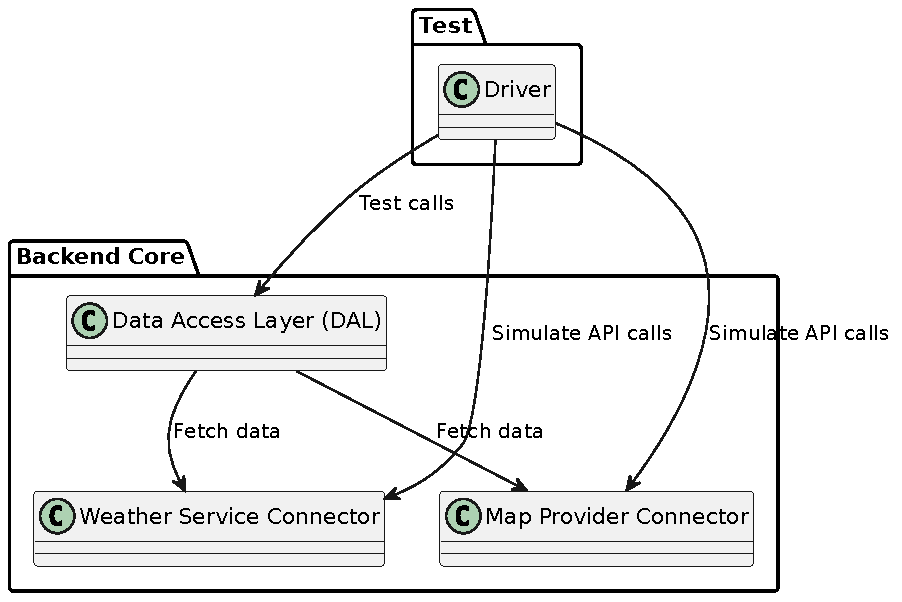
\includegraphics[width=0.6\textwidth]{Images/Integ_0.pdf}
    \caption{Integration Strategy - Step 0: Data Access \& Connectors}
    \label{fig:integration-strategy-step-0}
\end{figure}

\subsection{Step 1: User Management Foundation}
The \textbf{Users Account Manager Service} (implementing [F1] features) is integrated next. This service handles registration, authentication, and profile management, establishing the security foundation required for most system functionalities.

\begin{figure}[H]
    \centering
    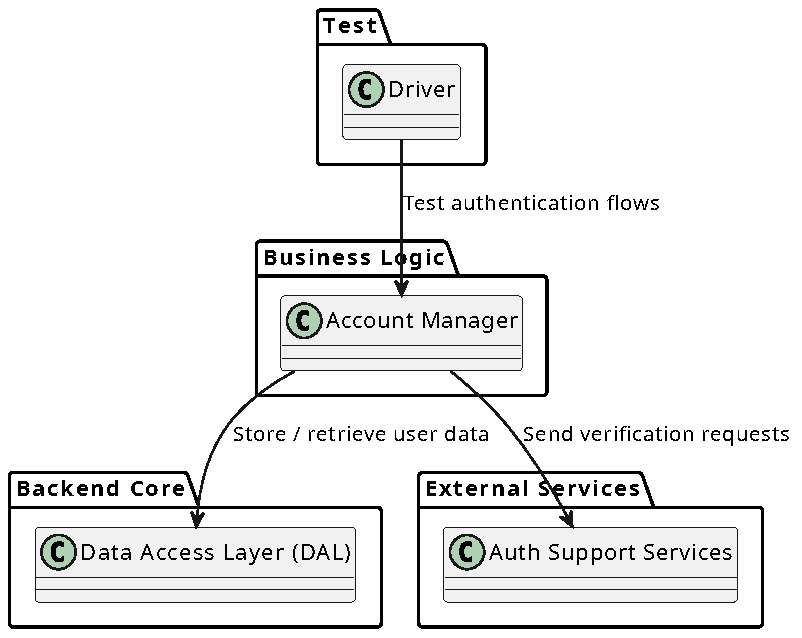
\includegraphics[width=0.6\textwidth]{Images/Integ_1.pdf}
    \caption{Integration Strategy - Step 1: Users Account Manager Service}
    \label{fig:integration-strategy-step-1}
\end{figure}

\subsection{Step 2: Core Processing Algorithms}
The \textbf{Sensor \& Detection Handler} ([F3]) and \textbf{Aggregation \& Scoring Engine} ([F5]) are implemented concurrently. These modules contain the system's core mathematical logic—anomaly detection and path scoring—which operate independently of user session state, ensuring algorithm robustness before UI integration.

\begin{figure}[H]
    \centering
    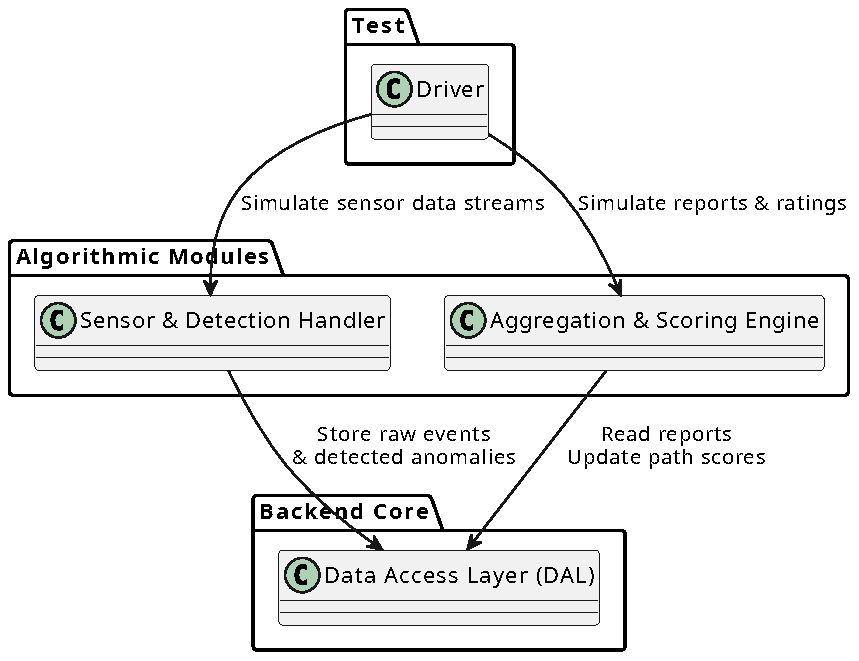
\includegraphics[width=0.6\textwidth]{Images/Integ_2.pdf}
    \caption{Integration Strategy - Step 2: Core Algorithms}
    \label{fig:integration-strategy-step-2}
\end{figure}

\subsection{Step 3: Trip and Reporting Orchestration}
The \textbf{Trip Ingestion Service} ([F2]) and \textbf{Report Server} ([F4]) are integrated as central orchestrators. The Trip Ingestion Service coordinates with the Users Account Manager (for user linkage), Sensor Handler (for data recording), and external adapters (for weather enrichment). The Report Server processes user submissions and interacts with the Aggregation Engine to update path statuses.

\begin{figure}[H]
    \centering
    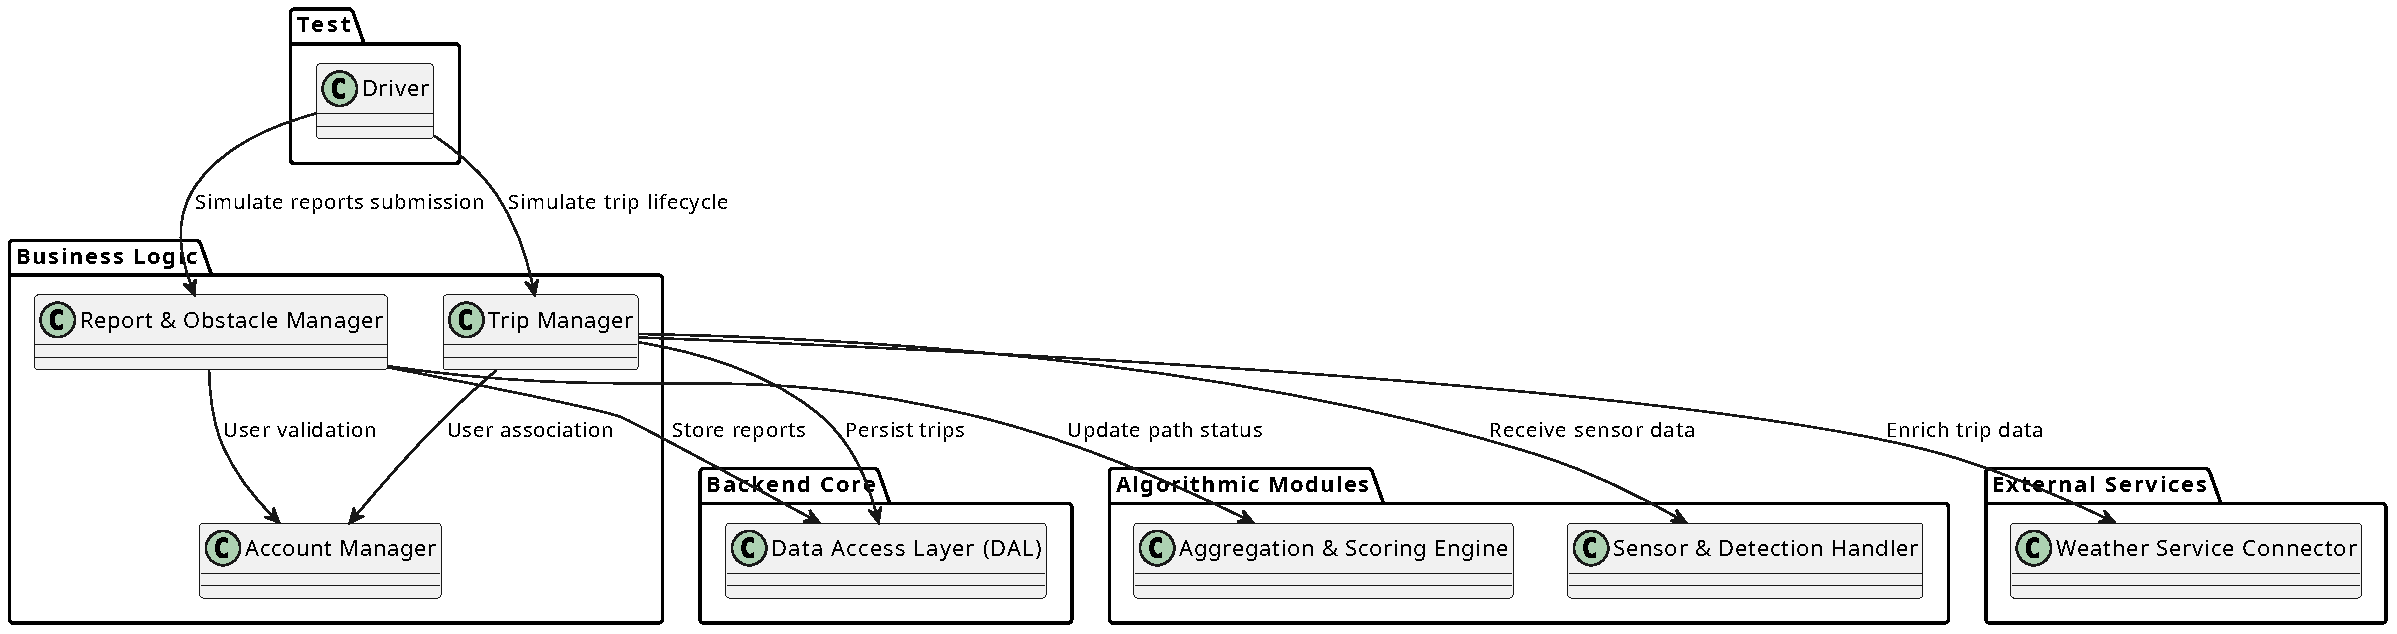
\includegraphics[width=1\textwidth]{Images/Integ_3.pdf}
    \caption{Integration Strategy - Step 3: Trip Ingestion and Report Services}
    \label{fig:integration-strategy-step-3}
\end{figure}

\subsection{Step 4: Search and Visualization Layer}
The \textbf{Trip Search Server} ([F6]) and \textbf{Dashboard Manager} ([F2/RU.9]) form the consumption layer. The Trip Search Server executes optimized queries over aggregated data, while the Dashboard Manager retrieves historical data for statistics visualization.

\begin{figure}[H]
    \centering
    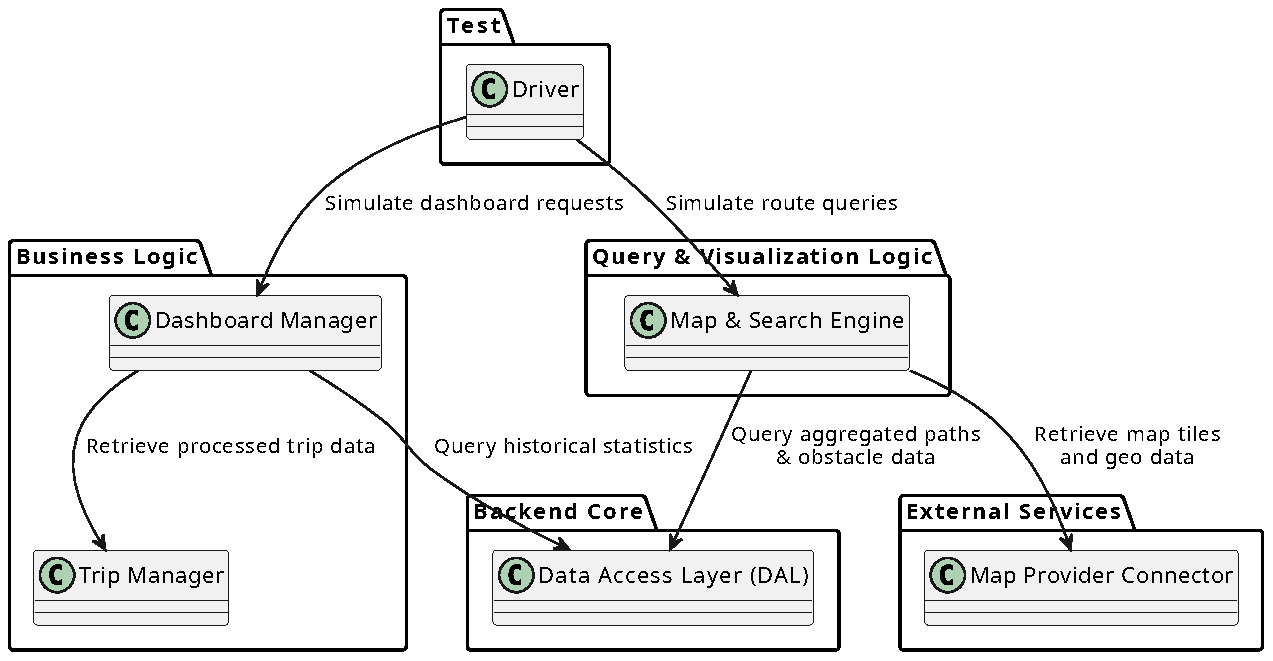
\includegraphics[width=0.8\textwidth]{Images/Integ_4.pdf}
    \caption{Integration Strategy - Step 4: Search and Dashboard}
    \label{fig:integration-strategy-step-4}
\end{figure}

\subsection{Step 5: Client Application Integration}
The final phase integrates client applications (Mobile App) with backend APIs. This validates end-to-end communication, JSON response handling, and interaction among client-side managers: Sensor Manager, Local Database Manager, Network Manager, and UI Controller.

\begin{figure}[H]
    \centering
    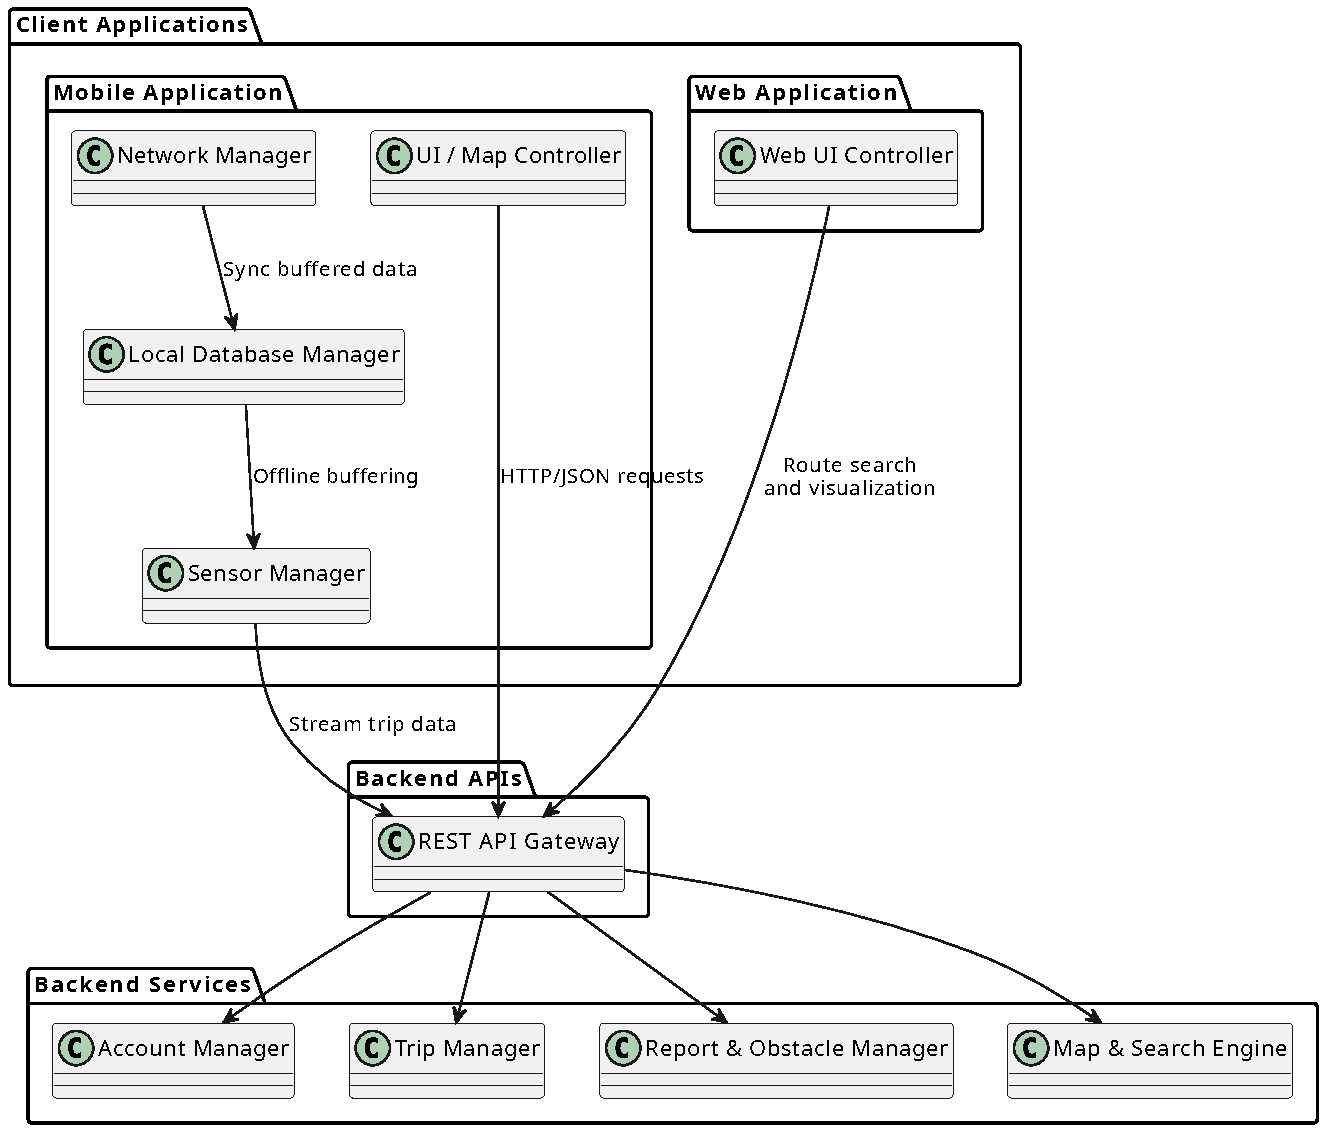
\includegraphics[width=0.8\textwidth]{Images/Integ_5.pdf}
    \caption{Integration Strategy - Step 5: Client Integration}
    \label{fig:integration-strategy-step-5}
\end{figure}

These client-side components correspond precisely to those defined in Section 2.2 (Architectural Design).

\section{System Testing Strategy}
\label{sec:system-testing-strategy}

Following component-level testing, the system undergoes comprehensive evaluation using a \textbf{Black-Box strategy}, assessing functionality from the user's perspective without internal implementation knowledge.

The testing regimen includes:

\begin{enumerate}
    \item \textbf{Functional Testing}: Validates that critical workflows (e.g., [RU.4] Automatic Trip Recording, [UU.2] Route Search) operate as specified in the RASD requirements.
    
    \item \textbf{Performance Testing}: Confirms the system handles expected loads of 50,000 active users, ensuring backend ingestion of high-frequency sensor data without latency and map rendering within 2 seconds.
    
    \item \textbf{Security Testing}: Verifies GDPR compliance for location data, ensures private trip isolation, and validates API endpoint resilience against SQL injection, token hijacking, and unauthorized access.
    
    \item \textbf{Failure Testing}: Simulates adverse conditions (GPS signal loss, network interruptions) to confirm graceful recovery and data preservation, addressing Constraint C05 (intermittent connectivity).
    
    \item \textbf{Endurance Testing}: Assesses system stability under prolonged use (e.g., 4-hour trip recording), checking for battery efficiency, resource leaks, and backend stability.
    
    \item \textbf{User Acceptance Testing (UAT)}: Real cyclists execute realistic tasks (riding varied terrains, reporting obstacles) to validate that the system meets practical needs and delivers satisfactory Quality of Experience (QoE).
\end{enumerate}